\documentclass{beamer}
\usepackage[utf8]{inputenc}
\usepackage[T1]{fontenc}
\usepackage{listings}
\usepackage{graphicx}
\usepackage{placeins}
\usetheme{Madrid}

\author{Renê Cardozo - 9797315 \\ 
        Verônica Stocco - 6828626 \\
        rene.cardozo@usp.br \\
        veronica.stocco@usp.br}

\title{EP2}
\institute{Instituto de Matemática e Estatística \\
Universidade de São Paulo}

\date{}

\begin{document}
\frame{\titlepage}

\begin{frame}

\frametitle{Corrida por eliminação}

O simulador é composto por dois módulos: aleatorio e pista. 
\begin{itemize}
\item \textbf{aleatorio} contém as funções responsáveis por determinar a velocidade e a probabilidade de quebra dos ciclistas.

\item \textbf{pista} contém o simulador em si, e será discutido em detalhe nos slides a seguir.

\end{itemize}
\end{frame}


\begin{frame}
\frametitle{Barreiras, turnos e pistas}

O simulador utiliza duas barreiras para gerenciar os turnos da simulação. Desta forma, enquanto as n threads ciclistas restantes aguardam em uma barreira, a barreira referente ao turno seguinte é criada. A operaçao das threads em \textbf{void ciclista()} é feita considerando esses dois possíveis turnos (par e ímpar).

Também foi utilizada uma barreira adicional para definir a largada das threads.

A pista é composta por 10 linhas (é possivel editar esse valor em pista.h). Cada linha tem \textbf{d} metros, e um \textbf{mutex\_pos} referente a cada metro / faixa da linha.  No início da simulação, os ciclistas são distribuídos nas linhas 0, 2, 4, 6 , 8.

\end{frame}



\begin{frame}
\frametitle{Ultrapassagem}

A cada rodada, a posição atual do ciclista é atualizada com \textbf{atualiza\_posicao}. Para evitar conflitos, são usados 4 mutex, referentes à:

\begin{itemize}
\item linha na qual o ciclista se encontra no momento;
\item linha para a qual o ciclista pode se mudar caso ocorra uma ultrapassagem;
\item próxima faixa (posição) que o ciclista pode ocupar na linha atual;
\item próxima faixa (posição) que o ciclista pode ocupar caso ocorra uma ultrapassagem;
\end{itemize}

\end{frame}



\begin{frame}
\frametitle{Eliminação de ciclistas}
A eliminação de ciclistas se dá de duas formas:

\begin{itemize}
\item \textbf{Por quebra:} a chance de quebra é definida aleatóriamente, conforme as especificações do enunciado.
\item \textbf{Por ser o último:} o último ciclista a completar uma volta de número par recebe uma flag em seu ID no vetor \textbf{elimina\_id}. Essa marcação occore no main. A eliminação é executada pela thread referente a esse ID, quando ela for executada. 
\end{itemize}

Quando um ciclista é eliminado, trancam-se os mutex ferentes à linha e faixa que ele ocupava para marcar essa posição como estando livre. Sua colocação é adicionada ao ranking, e outro mutex é utilizado para garantir que apenas uma thread altere o ranking de cada vez.
\end{frame}




\begin{frame}
\frametitle{Ranqueamento}
Optou-se por implementar 2 rankings distintos.


\begin{itemize}
\item \textbf{Ranking a cada rodada:} registra, no ID de cada ciclista, a sua colocação atual. Paralelo a esse ranking, um vetor de ints atômicos \textbf{pos\_volta} é utilizado para armazenar a posição do último corredor de cada volta.

\item \textbf{Ranking final:} conforme cada ciclista é eliminado, armazena-se sua colocação final na corrida, assim como tempo total, última volta e se sua bicicleta quebrou ou não.   
\end{itemize}

As atualizações nos valores dos rankings sempre são feitas utilizando mutexes referentes a eles.
\end{frame}




\begin{frame}
\frametitle{Bugs conhecidos}
O simulador apresenta alguns bugs que não conseguimos corrigir a tempo da entrega. 

\begin{itemize}
\item \textbf{n < 30}: o ranking é impresso, mas a execução do simulador precisa ser interrompida manualmente. Algumas vezes as informações do último ciclista não são devidamente registradas, e o programa imprime que seu tempo e total de volta foram 0.

\item \textbf{n > 30}: o simulador funciona como esperado até restarem em torno de 8 ciclistas na corrida. Quando isso acontece, não ocorrem mais eliminações. Os ciclistas remanescentes ficam ativos em loop até que o simulador seja interrompido manualmente.

\end{itemize}

\end{frame}


\begin{frame}
\frametitle{Máquinas Utilizadas}



\end{frame}

\begin{frame}
\frametitle{Gráficos: 10, 30, 100 ciclistas}


\begin{figure}[!htb]
\minipage{0.5\textwidth}
  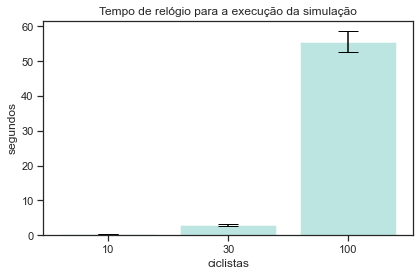
\includegraphics[width=\linewidth]{imgs/ciclistas_tempo}
  \caption{Tempo de execução}\label{fig:awesome_image1}
\endminipage\hfill
\minipage{0.5\textwidth}
  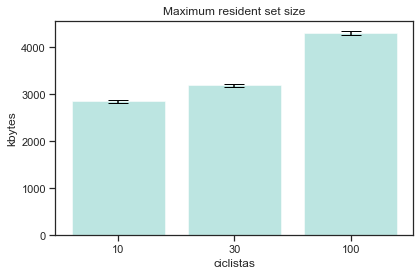
\includegraphics[width=\linewidth]{imgs/ciclistas_memoria}
  \caption{Uso de memória}\label{fig:awesome_image2}
  \endminipage\hfill
\end{figure}



\end{frame}


\begin{frame}
\frametitle{Gráficos: 10, 30, 100 ciclistas}
\begin{figure}[!htb]

\minipage{0.50\textwidth}%
  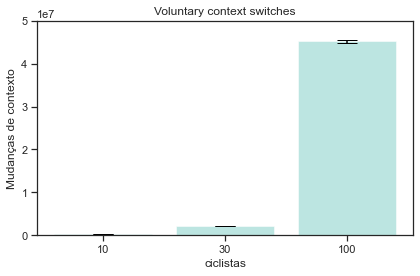
\includegraphics[width=\linewidth]{imgs/ciclistas_contexto}
  \caption{Mudanças de contexto}\label{fig:awesome_image3}
\endminipage

\end{frame}



\begin{frame}
\frametitle{Análise dos resultados}


\end{frame}


\end{document}

